%%%%%%%%%%%%%%%%%%%%%%%%%%%%%%%%%%%%%%%%%
% Thin Sectioned Essay
% LaTeX Template
% Version 1.0 (3/8/13)
%
% This template has been downloaded from:
% http://www.LaTeXTemplates.com
%
% Original Author:
% Nicolas Diaz (nsdiaz@uc.cl) with extensive modifications by:
% Vel (vel@latextemplates.com)
%
% License:
% CC BY-NC-SA 3.0 (http://creativecommons.org/licenses/by-nc-sa/3.0/)
%
%%%%%%%%%%%%%%%%%%%%%%%%%%%%%%%%%%%%%%%%%

%----------------------------------------------------------------------------------------
%	PACKAGES AND OTHER DOCUMENT CONFIGURATIONS
%----------------------------------------------------------------------------------------

\documentclass[a4paper, 10pt]{article} % Font size (can be 10pt, 11pt or 12pt) and paper size (remove a4paper for US letter paper)

\usepackage[protrusion=true,expansion=true]{microtype} % Better typography
\usepackage{graphicx} % Required for including pictures
\usepackage{wrapfig} % Allows in-line images
\usepackage{hyperref}

\usepackage[utf8]{inputenc}
\usepackage[T1]{fontenc}

\usepackage{mathpazo} % Use the Palatino font
\usepackage[T1]{fontenc} % Required for accented characters
\linespread{1} % Change line spacing here, Palatino benefits from a slight increase by default


\usepackage[top=1in, bottom=1.25in, left=1.25in, right=1.25in]{geometry}

\makeatletter
\renewcommand\@biblabel[1]{\textbf{#1.}} % Change the square brackets for each bibliography item from '[1]' to '1.'
\renewcommand{\@listI}{\itemsep=0pt} % Reduce the space between items in the itemize and enumerate environments and the bibliography

\renewcommand{\maketitle}{ % Customize the title - do not edit title and author name here, see the TITLE block below
\begin{flushright} % Right align
{\LARGE\@title} % Increase the font size of the title

\vspace{50pt} % Some vertical space between the title and author name

{\large\@author} % Author name
\\\@date % Date

\vspace{40pt} % Some vertical space between the author block and abstract
\end{flushright}
}

%----------------------------------------------------------------------------------------
%	TITLE
%----------------------------------------------------------------------------------------

\title{Sujet de stage Master ATIAM 2015-2016\\ % Title
\textbf{Représentation symbolique de musique orchestrale pour les méthodes d'apprentissage automatiques}} % Subtitle

\author{\textsc{Philippe Esling et Léopold Crestel} % Author
\\{\textit{IRCAM}}} % Institution

\date{8 Février 2016} % Date

%----------------------------------------------------------------------------------------

\begin{document}

\maketitle % Print the title section

%----------------------------------------------------------------------------------------
%	ABSTRACT AND KEYWORDS
%----------------------------------------------------------------------------------------

\hspace*{3,6mm}\textit{Keywords:} \textit{Deep learning}, \textit{Representation learning}, \textit{embedding space}, \textit{Music generation}

\vspace{30pt} % Some vertical space between the abstract and first section

%----------------------------------------------------------------------------------------
%	ESSAY BODY
%----------------------------------------------------------------------------------------

\section*{Contexte}

Depuis 2015, l'Institut de Recherche et Coordination Acoustique/Musique (\href{http://www.ircam.fr/}{IRCAM}) est engagé au côté de la Schulich School of Music de l'université McGill à Montréal (\href{http://www.mcgill.ca/music/}{SSM}) et de la Haute École de Musique de Genève	(\href{http://www.hesge.ch/hem/}{HEM}) dans un projet de recherche dont le but est de construire une théorie moderne de l'orchestration musicale. L'orchestration musicale peut se définir de manière générale comme l'art d'écrire des partitions musicales pour des ensembles d'instruments. L'un des objectifs de ce projet est de développer un système d'orchestration projective automatique dans lequel une partition pour piano est \textit{projetée} sur une partition d'orchestre. 
Ainsi, les différentes notes présentes dans la partition pour piano sont affectés à différents plan de timbre \cite{mcadams2013timbre} en conservant la structure harmonique, rythmique et mélodique.

Les récentes avancées en apprentissage automatique laissent entrevoir des résultats prometteurs (génération de séquences vidéos avec contexte \cite{taylor2009factored}). Parmi la grande famille des réseaux de neurones, certains modèles probabilistes génératifs offrent un cadre élégant pour appréhender ce problème et les outils adaptés pour le résoudre. Si le terme réseaux de neurones regroupe un nombre important de modèles en pratique diffèrent, tous ont pour principe fondateur l'inférence statistique de régularités (i.e. corrélations) dans un ensemble de données. Dans le cadre de l'orchestration automatique il s'agit de comprendre les mécanismes sous-jacent en observant des exemples d'orchestrations réalisées par de grands compositeurs. Ces exemples d'orchestrations sont appelés dans un cadre plus général \textit{base d'entraînement}. La qualité du modèle dépend grandement de la qualité et du nombre d'exemples contenus dans la base d'entraînement.

En informatique musicale, on oppose souvent données symboliques (la partition d'orchestre) et données du signal (\textit{e.g.} enregistrement audio). Si nous pensons qu'un système d'orchestration ne peut se contenter uniquement de l'une des deux modalités, nous nous focalisons dans un premier temps sur un modèle entraîné avec des données purement symboliques. Les données musicales symboliques peuvent être représentées de nombreuses manières. En informatique et dans un cadre algorithmique, le format traditionnellement utilisé est celui du \textit{piano-roll} (\textit{cf} figure \ref{refpr}). La série temporelle formée par les colonnes du \textit{piano-roll} peut être utilisée comme donnée d'entraînement pour un réseau de neurone.
\begin{figure}
\begin{center}
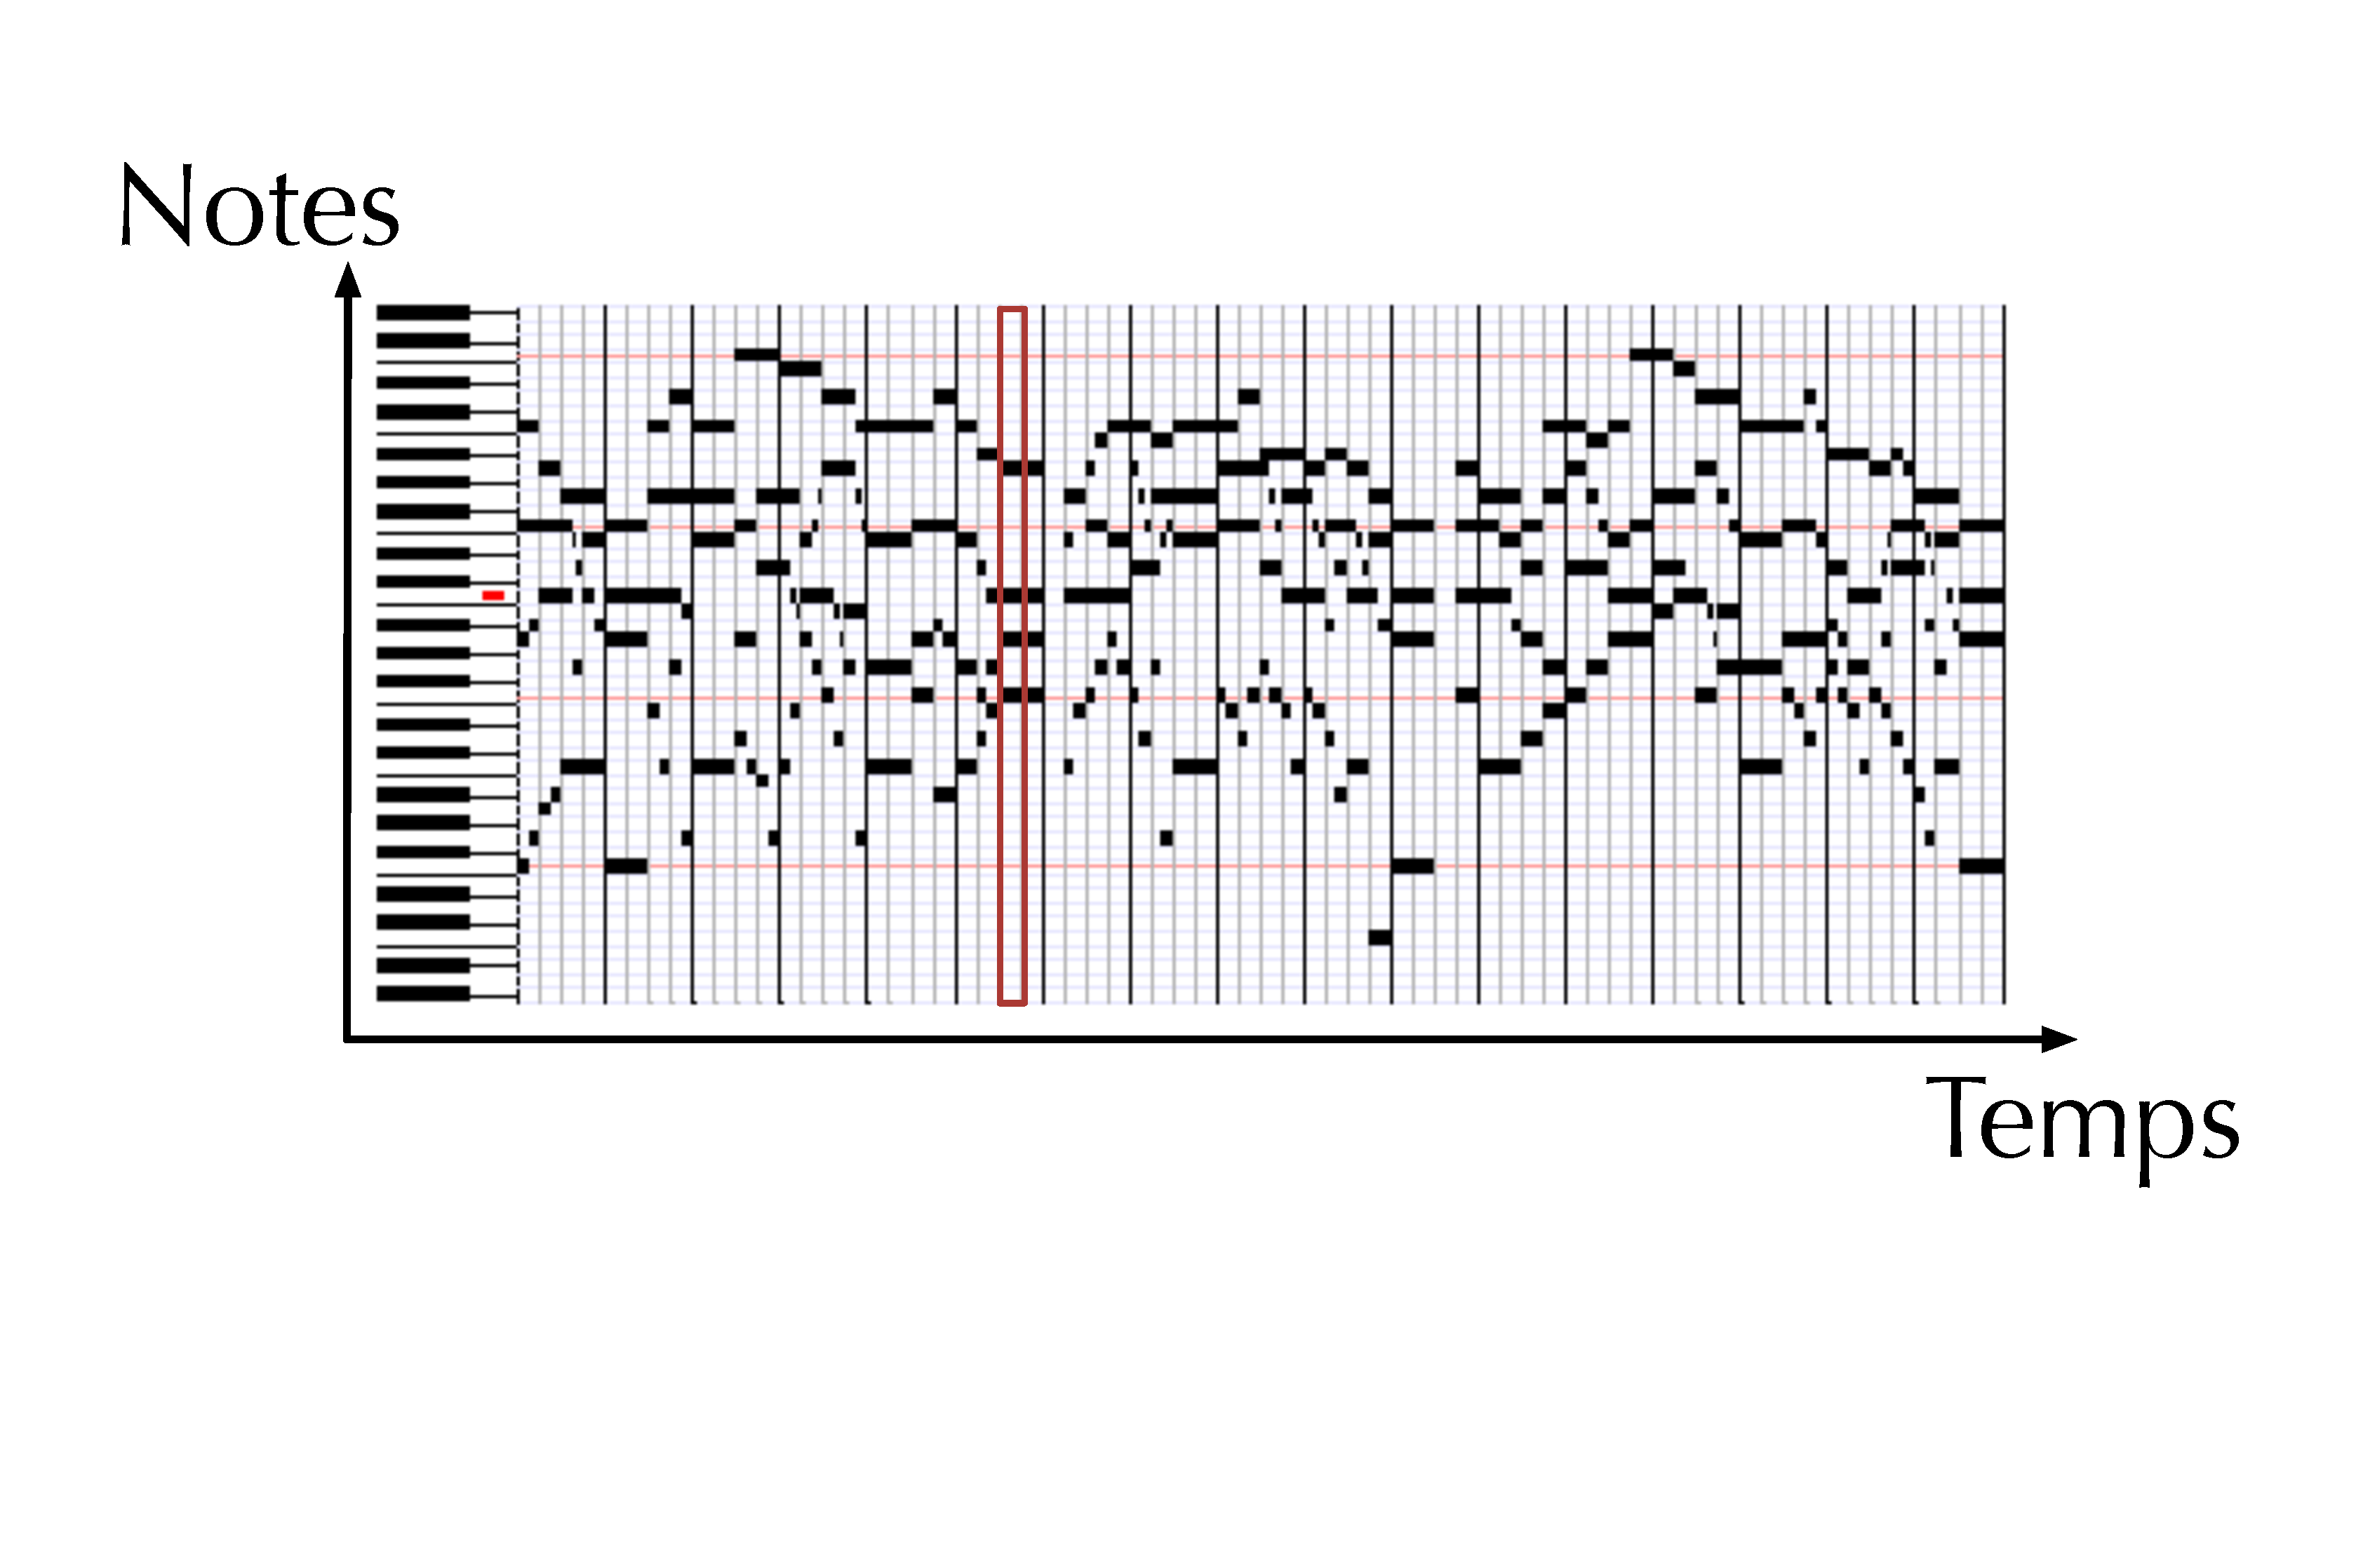
\includegraphics[scale=0.25]{../pr.pdf}
\caption{Représentation \textit{piano-roll}. Le temps est discrétisé selon un quantum de temps de référence (typiquement une fraction de la noire). Les fréquences sont discrétisées selon le tempérament égal en vigueur dans la musique classique occidentale (12 notes de DO à SI et une octave). Le \textit{piano-roll} est une matrice $P$ binaire dont la valeur $P(n,t)$ est égale à 1 si la note $n$ est jouée à l'instant $t$ et à 0 sinon.}
\label{refpr}
\end{center}
\end{figure}

\section*{Problématiques : manque de données et parcimonie}
La collecte de données est essentielle en vue de construire un modèle d'orchestration automatique performant. Deux difficultés surgissent lors de la construction d'une base de données symboliques pour l'orchestration : la taille des bases de données et la nature parcimonieuse des vecteurs manipulés.

Plus le nombre de données d'entraînement est grand et meilleur sera le modèle. Recopier au format numérique (MIDI ou XML) des partitions d'orchestre est fastidieux et peu de compositeurs se sont attelés à cette tâche. La première difficulté est donc la relative paucité de base de donnée de qualité et taille suffisantes.

Par ailleurs, la représentation en \textit{piano-roll} découle d'une discrétisation du temps et de la hauteur des fréquences certes naturelle, mais peu adaptée aux techniques d'apprentissage que nous souhaitons utiliser. Si on considère un d'orchestre composé d'une vingtaine de pupitres différents, chacun pouvant jouer 40 hauteurs de notes différentes, on obtient à chaque instant un vecteur de taille 800 ne contenant qu'une vingtaine de coordonnées non nulles. Seul une faible partie de l'ensemble possible de ces vecteurs sera contenu dans la base de départ.

\section*{Sujet de stage}
\begin{figure}
\begin{center}
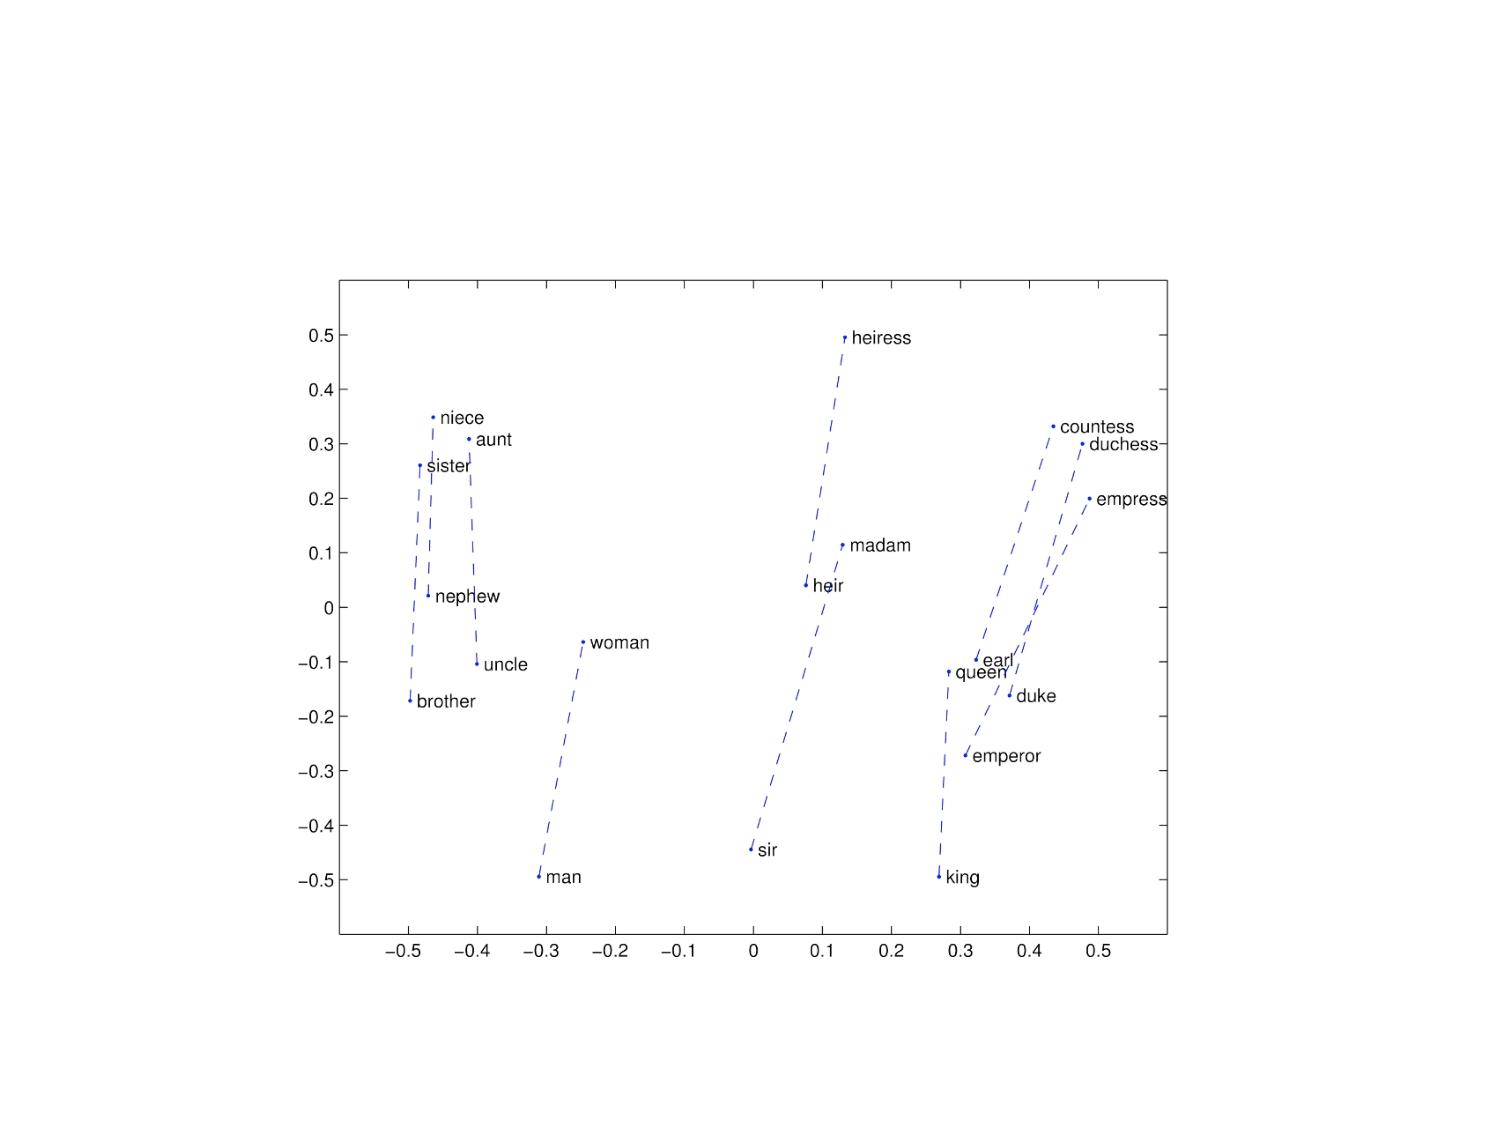
\includegraphics[scale=0.4]{../word_embedding.pdf}
\caption{Visualisation de la projection sur 2 dimensions d'un espace de plongement (\textit{embedding)} pour des vecteurs de mots selon des axes associés au genre \cite{pennington2014glove}}
\label{fig:word-embedding}
\end{center}
\end{figure}
Nous proposons de mener au cours de ce stage une réflexion sur les différentes manières de représenter l'information contenue dans une partition pour orchestre. Les deux problématiques soulevées précédemment engagent ainsi deux axes de recherches principaux :
\begin{description}
\item[\textit{Data augmentation}] : Fréquemment employée en reconnaissance d'image, cette technique consiste à appliquer des transformations et dégradations sur les données de la base d'entraînement afin d'en augmenter artificiellement la taille. En image, ces transformations sont généralement des obstructions (mise à zéro d'une partie des pixels de l'image), changement d'échelle, transvections (\textit{shear mapping}). Quelles seraient ces transformations pour la musique orchestrale ? 
%Les transpositions viennent immédiatement à l'esprit, mais de combien de notes ?
\item[\textit{Chord-embedding}] : une représentation "naïve" des mots en traitement du langage naturel consiste à prendre un vecteur de la taille du dictionnaire étudié et associer chaque dimension à un mot (\textit{one-hot encoding}). En anglais, pour un dictionnaire restreint de 30000 mots, chaque mot est alors représenté par un vecteur de taille 30000 constitué uniquement de zéro sauf pour une coordonnée égale à 1, ce qui est extrêmement parcimonieux. Une solution consiste alors à encoder les vecteurs dans un espace de dimension plus petit que l'espace de départ. Cet espace est appelé dans la littérature \textit{embedding} \cite{mikolov2013distributed}, et peut être recherché de manière automatique en fixant comme objectif la prédiction du contexte entourant le mot (cf figure \ref{fig:word-embedding}). Les espaces ainsi construits exhibent généralement d'intéressantes relations entre transformations géométriques et valeur sémantique. Pour de nombreuses raisons (similitude entre les différents instruments, intensité des notes, simultanéité de leurs occurrences dans la musique polyphonique) l'analogie avec le langage est limitée, et il ne s'agira pas d'effectuer une simple adaptation des techniques utilisées en traitement du langage naturel, mais de proposer une méthode spécifiquement ciblée à la nature des données orchestrales.
\end{description}

\section*{Déroulement du stage et compétences requises}
Le stage s'étend sur une durée de 2 mois à plein-temps, aménageable sur 6 mois.
Le stage s'articulera ainsi autour de points de travail suivants :
\begin{itemize}
\item Data augmentation (2 semaines)
\begin{itemize}
\item Bibliographie des méthodes de \textit{data augmentation} utilisées en traitement d'image.
%% Pscho-ac, cognition pour les effets timbres ? Genre qule instrument modifier ?
\item Interview avec des compositeurs (transformations admissibles ?)
\item Proposition et implémentation d'un ensemble de transformations spécifiques à l'orchestration
\end{itemize}
\item Chord-embedding (1 mois et demi)
\begin{itemize}
\item Bibliographie des techniques employées en traitement du langage naturel \cite{mikolov2013distributed, DBLP:journals/corr/KirosZSZTUF15}
\item Développement et implémentation de plusieurs algorithmes de construction des espaces de enchâssement (\textit{embedding}) adaptés à l'orchestration.
\item Évaluation qualitative, en étudiant notamment l'effet de diverses transformations géométriques dans l'espace de enchâssement
\item Évaluation quantitative sur une tâche de prédiction à court-terme
\end{itemize}
\end{itemize}

Le candidat doit avoir de solides bases en informatique et mathématique. Une connaissance des méthodes d'apprentissage automatique est souhaitable.
Une bonne connaissance de la musique et si possible de la composition orchestrale est essentielle. Le langage de programmation utilisé est laissé libre, avec une préférence pour Matlab ou Python.


%----------------------------------------------------------------------------------------
%	BIBLIOGRAPHY
%----------------------------------------------------------------------------------------

\bibliographystyle{unsrt}
\bibliography{../biblio}

%----------------------------------------------------------------------------------------

\end{document}